%! Author = Niek Scholten
%! Date = 24-10-2022

%Turn off page numbering
\pagenumbering{gobble}
\begin{center}

    \Huge{Predicting bird species from their songs using machine learning}\\
    \vspace{\baselineskip}
    \LARGE{Theme 09 - Introduction Machine Learning}\\
    \large{Research paper}\\
    \vspace{\baselineskip}

    \begin{figure}
        \centering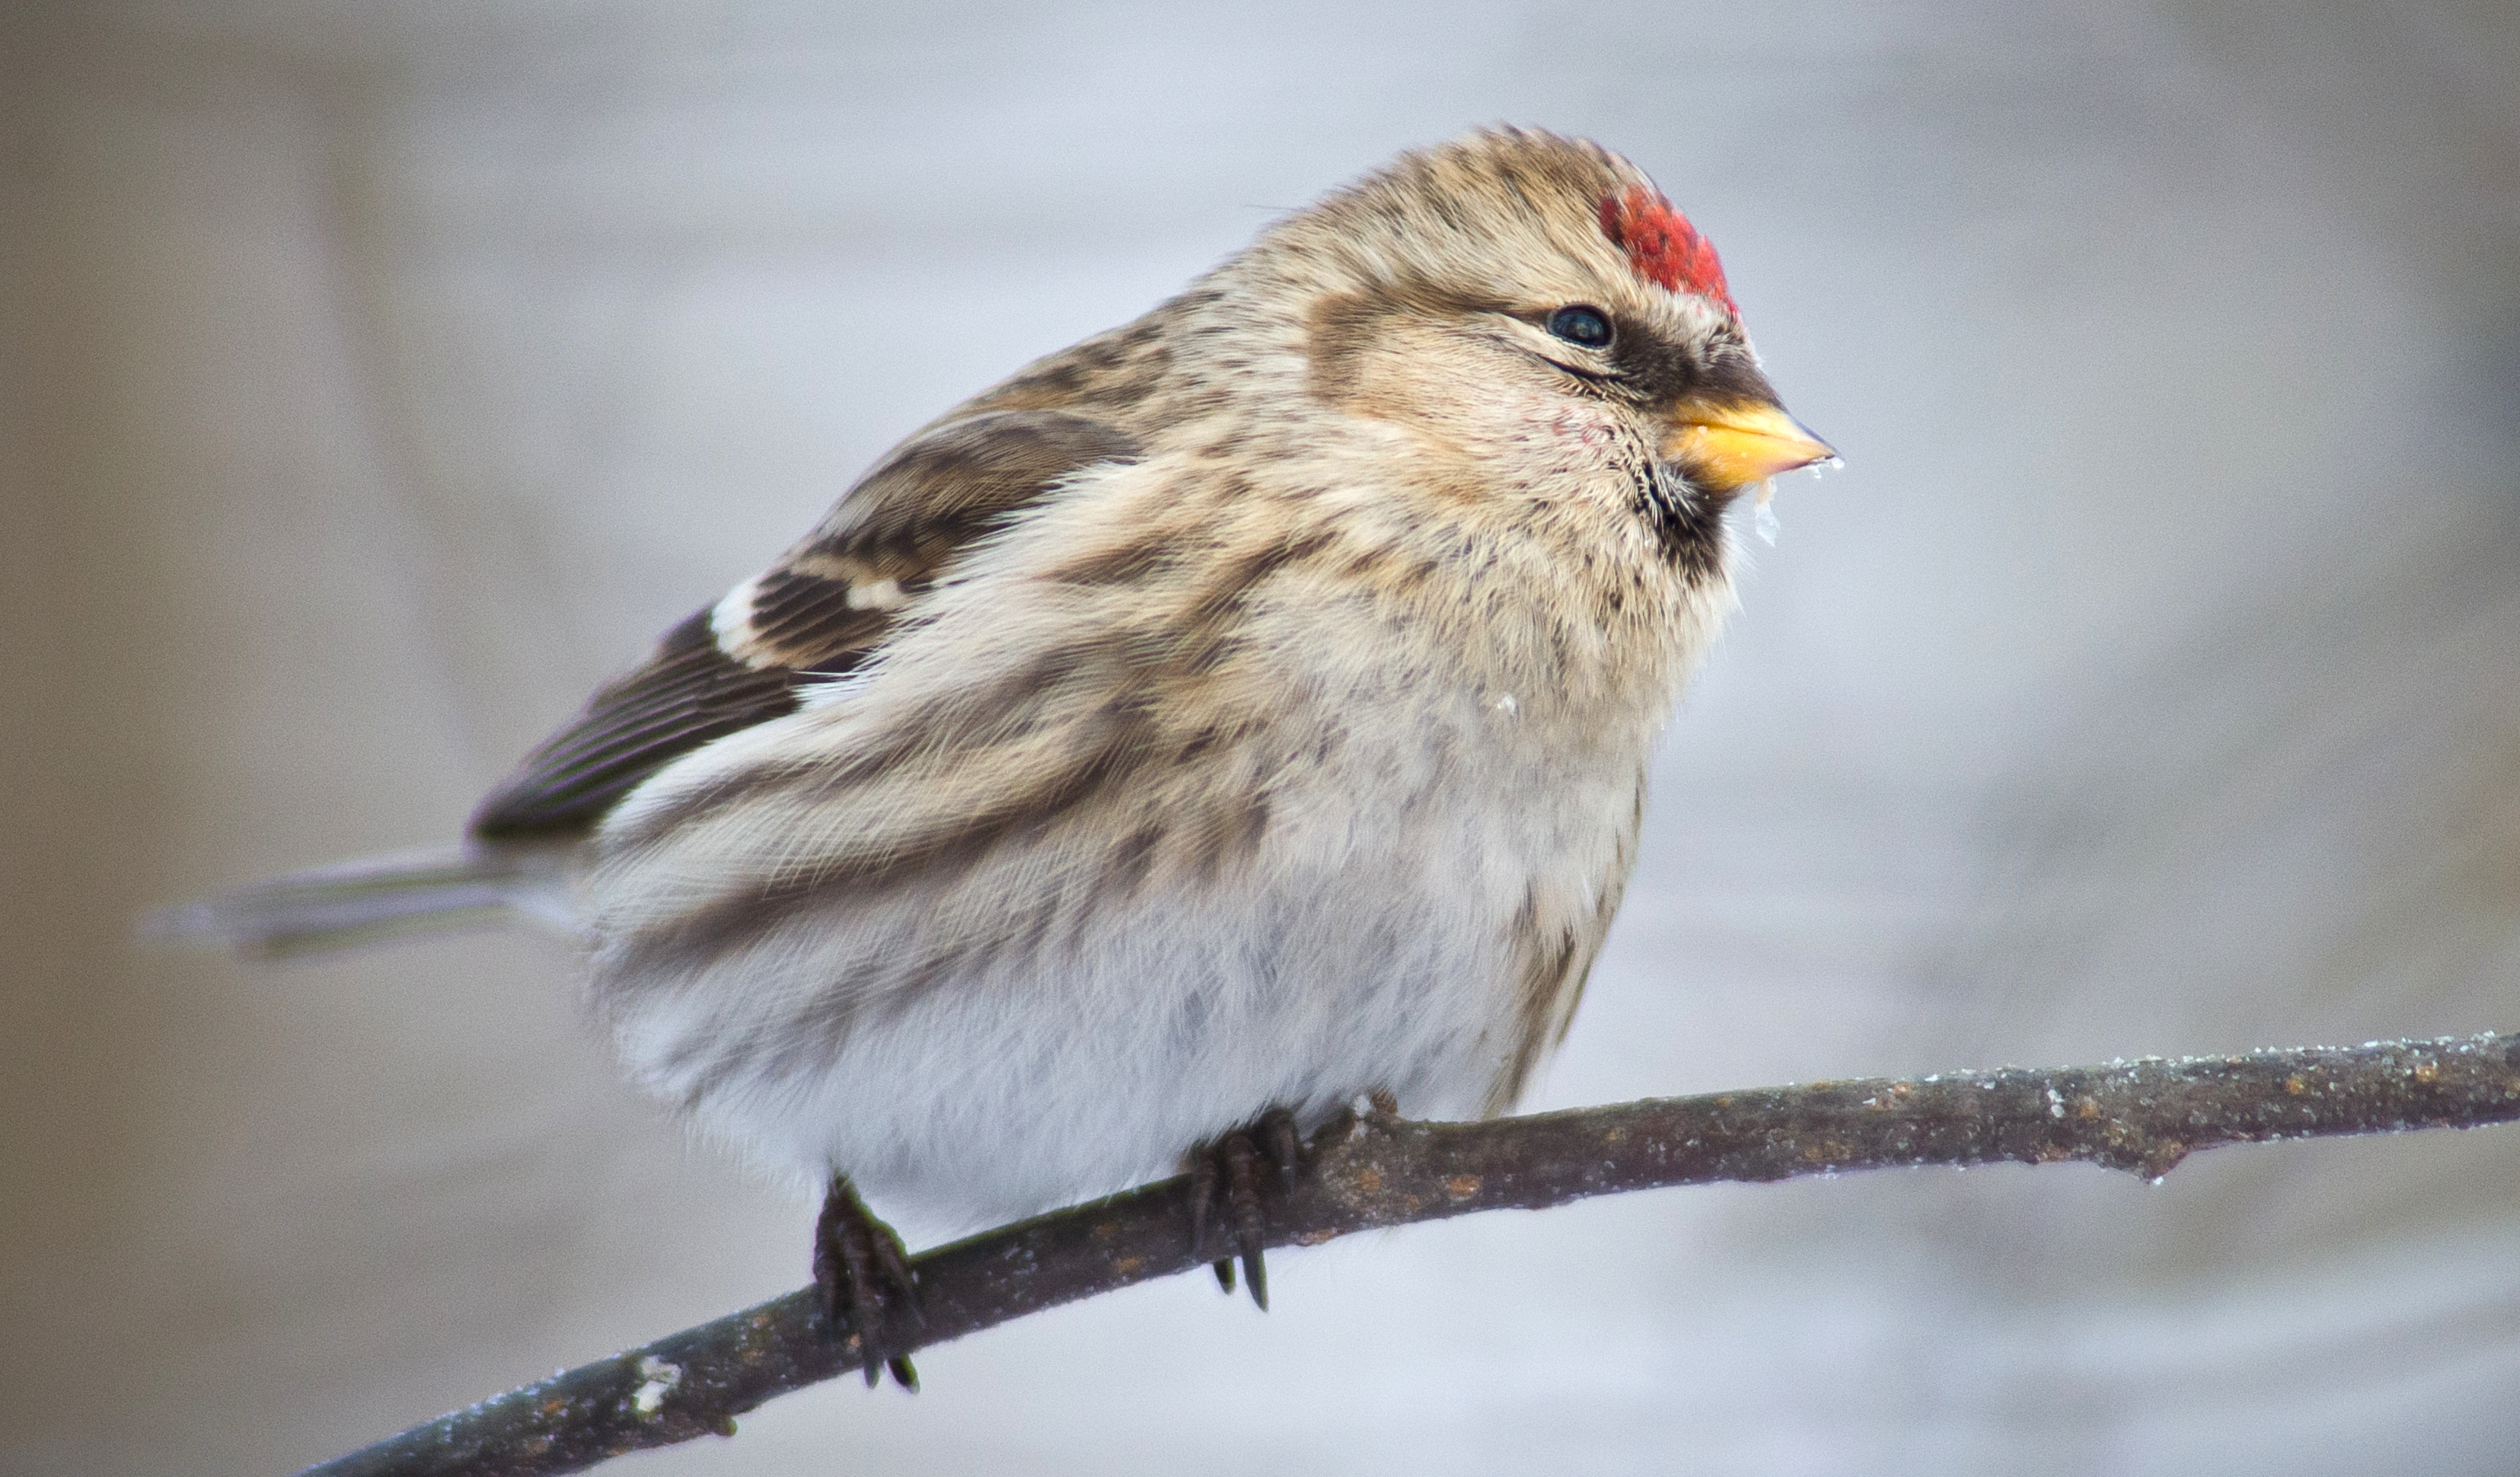
\includegraphics[width=\linewidth]{Acanthis_flammea}
        \caption{A common redpoll (Acanthis Flammea)}
        \label{fig:Acanthis_flammea}
    \end{figure}

\end{center}
\vspace{\baselineskip}

%Students info
\normalsize
\vspace*{\fill}
\begin{flushright}
    Niek R. Scholten (388602)\\
    Bio-Informatics BFV3\\
    Institute of Life Science \& Technology\\
    Hanze University of Applied Sciences\\
    Dave Langers (LADR) \& Bart Barnard (BABA)\\
    \today\\
    \href{https://github.com/niek265/Thema9-Praktijkopdracht}{From: https://github.com/niek265/Thema9-Praktijkopdracht}
\end{flushright}
\newpage

%Blank page
\null
\thispagestyle{empty}
\addtocounter{page}{-1}
\newpage

\begin{center}

%Titles

    \Huge{Predicting bird species from their songs using machine learning}\\
    \vspace{\baselineskip}
    \LARGE{Theme 09 - Introduction Machine Learning}\\
    \vspace{\baselineskip}

\end{center}
\vspace{\baselineskip}

%Students info
\normalsize
\vspace*{\fill}
\begin{flushright}
    Niek R. Scholten (388602)\\
    Bio-Informatics BFV3\\
    Institute of Life Science \& Technology\\
    Hanze University of Applied Sciences\\
    Dave Langers (LADR) \& Bart Barnard (BABA)\\
    \today\\
    \href{https://github.com/niek265/Thema9-Praktijkopdracht}{From: https://github.com/niek265/Thema9-Praktijkopdracht}
\end{flushright}
\newpage

\pagenumbering{roman}
\section*{Abstract}

The complexity and the consistency of birds' songs have long been marveled over.
And they always say ``consistency is key'', which is also true for the models in this project.
All the data that was used follows nice conventions and is perfect for machine learning.
This study aims to find out how well new songs of those same bird species can be classified using a model trained on the original data using machine learning.

\label{sec:abstract}~\addcontentsline{toc}{section}{\nameref{sec:abstract}}
\newpage

\section*{Summary}

Birds' songs can be complex and hard to distinguish by ear, but these songs can be easily transcribed to numeric data which is easily understood by computers.
The goal of this research is to create an easy to run program that can classify new instances of this numeric convention.
Python was used in pre-processing to make sure all data was structured correctly and ready for visualisation.
Weka was used after this to explore possible models for the dataset, the best model was chosen and exported to be used in a Java program.
The wrapper has been successfully built and can classify new instances with a high accuracy.

\label{sec:summ}~\addcontentsline{toc}{section}{\nameref{sec:summ}}
\newpage

\section*{List of Abbreviations}

\textbf{CSV} Comma-separated values

\textbf{STFT} Short-time Fourier transform

\label{sec:abvs}~\addcontentsline{toc}{section}{\nameref{sec:abvs}}

\newpage